\documentclass[crop,tikz]{standalone}
\usepackage{amsmath}
\usepackage{amsfonts}
\usepackage{physics}
\usepackage{tikz}
\usetikzlibrary{shapes}
\usepackage{dsfont}
\usepackage{bbm}
% parameters for the MPS drawings
\definecolor{Tcolor}{RGB}{255, 235, 171}
\definecolor{Wcolor}{RGB}{190, 190, 255}
\def\textoffsetVertical{0.8}
\def\nodewidth{0.6*28.5}
\def\legwidth{0.8}
\def\nodedistance{1.25}
\def\textoffsetVerticalW{0.9}
\def\textoffsetHorizontalW{-0.9}
\def\textoffsetVerticalMPO{1.2}
\def\yoffset{1}
\def\xoffset{3}
\def\resultMPSYoffset{2.5}
\def\resultMPSXOffsetSmall{2}
\def\resultMPSXOffset{3}
\def\dotsOffset{3}
\def\conjOffsetVertical{1.25}
\def\conjOffsetVerticalLarge{2.2}
\def\curvedLineXOffset{0.7}
\def\cmscale{28.5}
\def\miniatureScale{0.5}
\def\Heffheight{1.2*28.5}
\def\Heffwidth{4.0*28.5}
\def\Heffonewidth{3.0*28.5}
\def\miniatureTextOffsetVertical{0.5}
\begin{document}
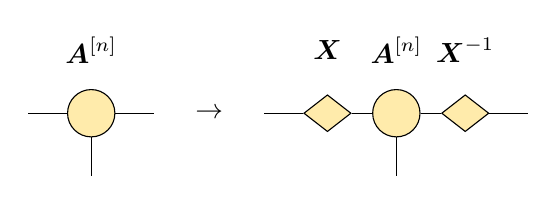
\begin{tikzpicture}[baseline=(current  bounding  box.center)]
    \node[draw, shape=circle, fill=Tcolor, minimum width=\nodewidth] (T1) at (0, 0) {};
    \node[] (text1) at (0, \textoffsetVertical) {$\vb*{A}^{[n]}$};
    \draw (T1) -- ++(-\legwidth, 0);
    \draw (T1) -- ++(0, -\legwidth);
    \draw (T1) -- ++(\legwidth, 0);
    \node[draw, shape=diamond, fill=Tcolor, minimum width=\nodewidth] (X1) at (\resultMPSXOffset, 0) {};
    \node[draw, shape=circle, fill=Tcolor, minimum width=\nodewidth] (T1p) at ({1*\nodedistance*0.7+\resultMPSXOffset}, 0) {};
    \node[draw, shape=diamond, fill=Tcolor, minimum width=\nodewidth] (Xm1) at ({2*\nodedistance*0.7+\resultMPSXOffset}, 0) {};
    \node[] (text2) at (0+\resultMPSXOffset, \textoffsetVertical) {$\vb*{X}$};
    \node[] (text3) at ({1*\nodedistance*0.7+\resultMPSXOffset}, \textoffsetVertical) {$\vb*{A}^{[n]}$};
    \node[] (text4) at ({2*\nodedistance*0.7+\resultMPSXOffset}, \textoffsetVertical) {$\vb*{X}^{-1}$};
    \draw (X1) -- ++(-\legwidth, 0);
    \draw (Xm1) -- ++(\legwidth, 0);
    \draw (X1) -- (T1p) -- (Xm1);
    \draw (T1p) -- ++(0, -\legwidth);
    \node[] (arrow) at (\resultMPSXOffset/2, 0) {$\rightarrow$};
\end{tikzpicture}
\end{document}